\documentclass[aspectratio=169]{beamer}
\usepackage{fontspec}
\usepackage{luatexja-fontspec}
\usepackage{graphicx}
\usepackage{tcolorbox}
\usepackage{xcolor}
\usepackage{amsmath}
\usepackage{amsfonts}
\usepackage{mathrsfs}
\usepackage{bm}
\usepackage{tikz}
\usepackage{booktabs}
\usepackage{url}
\usepackage{listings}
\usepackage{./theme/beamerthemeSimpleJapanese}


\everymath{\displaystyle}
\title[short title]{日本語のBeamerテンプレート}
\subtitle{Japanese Simple Beamer Template}
\author[sakikuroe]{KUROE Saki (黒江紗希)}
\institute[Hoge大]{Hogehoge University}
\date{\today}

\begin{document}

\begin{frame}
    \titlepage
\end{frame}

\begin{frame}{目次}
    \tableofcontents
\end{frame}

\section{概要}
\begin{frame}{概要}
    日本語で Beamer を使用するためのテンプレートです。
\end{frame}

\section{数式}
\begin{frame}{数式 (級数、積分、極限)}
    $$\sum_{n=1}^{\infty} \frac{1}{n^{2}} = 1 + \frac{1}{2^{2}} + \frac{1}{3^{2}} + \cdots = \frac{\pi^{2}}{6}$$
    $$\int_{0}^{\infty}e^{-ax^{2}}dx=\frac{1}{2}\sqrt{\frac{\pi}{a}}$$
    $$\lim_{n\rightarrow\infty}\frac{\sin x}{x}=1$$
\end{frame}

\begin{frame}{数式 (様々な文字)}
    \begin{itemize}
        \item ローマン体 : $\mathrm{ABCDEFGHIJKLMNOPQRSTUVWXYZ}$
        \item サンセリフ体 : $\mathsf{ABCDEFGHIJKLMNOPQRSTUVWXYZ}$
        \item 太字 : $\bm{ABCDEFGHIJKLMNOPQRSTUVWXYZ}$
        \item 黒板太字 : $\mathbb{ABCDEFGHIJKLMNOPQRSTUVWXYZ}$
        \item 筆記体 : $\mathcal{ABCDEFGHIJKLMNOPQRSTUVWXYZ}$
        \item 花文字 : $\mathscr{ABCDEFGHIJKLMNOPQRSTUVWXYZ}$
        \item ギリシャ文字 : $\alpha\beta\gamma\delta\epsilon\varepsilon\zeta\eta\theta\vartheta\iota\kappa\lambda\mu\nu\xi o\pi\varpi\rho\varrho\sigma\varsigma\tau\upsilon\phi\varphi\chi\psi\omega$
        \item ドイツ文字 : $\mathfrak{ABCDEFGHIJKLMNOPQRSTUVWXYZ}$
    \end{itemize}
\end{frame}

\begin{frame}{数式 (行列)}
    $$
        A
        =
        \begin{bmatrix}
            a_{11} & a_{12} & \dots  & a_{1m} \\
            a_{21} & a_{22} & \dots  & a_{2m} \\
            \vdots & \vdots & \ddots & \vdots \\
            a_{n1} & a_{n2} & \dots  & a_{nm}
        \end{bmatrix}
    $$
\end{frame}

\begin{frame}{数式 (定理環境)}
    \begin{tcolorbox}[
            colback=white,
            sharp corners,
            toprule=0pt,
            bottomrule=0pt,
            rightrule=0pt,
            leftrule=3pt,
        ]
        \textbf{Def. 1.1 (\textcolor{Red}{\bf{完全加法族}})}%
        \tcblower
        \begin{tcolorbox}[
                colback=white,
                sharp corners,
            ]
            \begin{itemize}
                \item $S$: 集合
                \item $\mathcal{F} \in 2^{S}$
            \end{itemize}
        \end{tcolorbox}
        $\mathcal{F}$が\textcolor{Red}{\bf{完全加法族}} \\
        $\overset{\mathrm{def}}{\Longleftrightarrow}$
        \begin{enumerate}
            \item $\varnothing \in \mathcal{F}$
            \item $A \in \mathcal{F} \Rightarrow A^{c} \in \mathcal{F}$
            \item $\{A_{i}\}_{i=1}^{\infty} \subset \mathcal{F} \Rightarrow \bigcup_{i=1}^{\infty} A_{i} \in \mathcal{F}$
        \end{enumerate}
    \end{tcolorbox}
\end{frame}

\section{Tikz}
\begin{frame}{Tikz}
    \begin{center}
        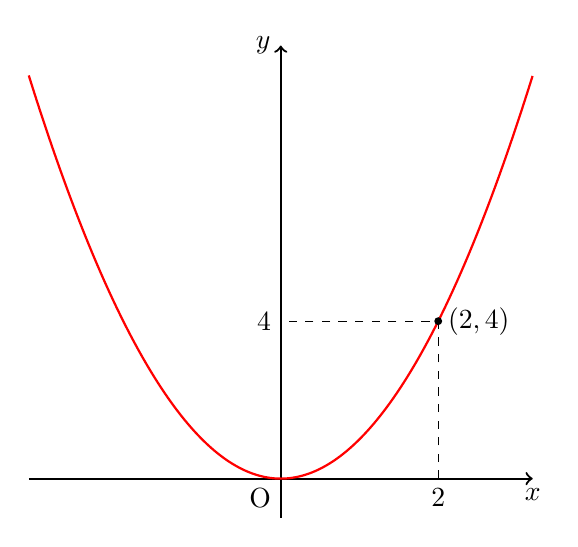
\begin{tikzpicture}[xscale=1.0,yscale=0.5]
            \draw[thick,->] (-3.2,0.) -- (3.2,0.) node[below] {$x$};
            \draw[thick,->] (0,-1.) -- (0,11.) node[left] {$y$};
            \draw (0.,0.) node[below left] {$\mathrm{O}$} coordinate;
            \draw (2.,0.) node[below] {$2$} coordinate;
            \draw (0.,4.) node[left] {$4$} coordinate;
            \draw [Red,domain=-3.2:3.2,thick,samples=200] plot(\x,{pow(\x, 2.0)});
            \draw (2.,4.) node[right] {$(2,4)$};
            \fill[xscale=0.5,yscale=1.0] (4.,4.) circle(0.1);
            \draw [dashed](2.,0.)--(2.,4.)--(0.,4.);
        \end{tikzpicture}
    \end{center}
\end{frame}

\section{図表}
\begin{frame}{図}
    \begin{figure}[htbp]
        \begin{center}
            \includegraphics[scale=0.02]{figure/mandelbrot.png}
            \caption{マンデルブロ集合}
        \end{center}
    \end{figure}
\end{frame}

\begin{frame}{表}
    \begin{table}[H]
        \caption{日本語と英語の対応}
        \label{table:ja-en}
        \begin{tabular}{lll}
            \toprule
            ひらがな & 漢字 & 英語   \\
            \midrule
            りんご   & 林檎 & apple  \\
            みかん   & 蜜柑 & orange \\
            ぶどう   & 葡萄 & grape  \\
            \bottomrule
        \end{tabular}
    \end{table}
\end{frame}

\section{箇条書き}
\begin{frame}{箇条書き (番号有り)}
    \begin{enumerate}
        \item A
        \item B
        \item C
        \item D
        \item E
    \end{enumerate}
\end{frame}

\begin{frame}{箇条書き (番号無し)}
    \begin{itemize}
        \item A
        \item B
        \item C
        \item D
        \item E
    \end{itemize}
\end{frame}

\section{コードブロック}
\begin{frame}[fragile]{コードブロック}
    \begin{lstlisting}[
        frame={tb},
        language=c,
        numbers=left,
        caption=hello\_world.c,
        showspaces=false,
        showstringspaces=false,
        xrightmargin=0.05\textwidth,
        xleftmargin=0.05\textwidth,
    ]
#include<stdio.h>

int main(void) {
    printf("Hello world!\n");
    return 0;
}
    \end{lstlisting}
\end{frame}

\end{document}